\chapter{Transformasi Digital}
\label{ch:transformasi-digital}

Digitalisasi, digambarkan dengan sederhana oleh KBBI sebagai proses pemberian atau pemakaian yang sistem yang berkaitan dengan komputer atau internet. Bayangkan dulu (atau bahkan hingga sekarang) sebuah toko kelontong yang melayani ratusan pembeli setiap harinya, bagaimana repotnya mencatat transaksi keluar masuk barang dengan buku dan pena dan nota dalam bentuk tulisan di lembaran kardus bekas. Mungkin belum terlihat sebagai masalah, Namun ketika waktu rekapitulasi untung dan rugi atau ketika ada pelanggan yang komplain maka disitulah pening kepala pemilik toko kelontong.

Digitalisasi membawa kemudahan yang luar biasa bagi seluruh sendi kehidupan kita, jika dilanjutkan pada lingkup toko kelontong tadi, maka kita jumpai minimarket dengan sistemnya mampu mencatat inventori barang dan memberikan nota pembelian sekaligus secara cepat dan akurat. Walaupun digitalisasi juga membawa dampak buruk seperti, janji-janji penting yang dapat dibatalkan hanya dalam sebuah pesan singkat saja. Terlepas dari hal tersebut digitalisasi tidak hanya memudahkan pemilik toko kelontong kesayangan kita akan tetapi dunia pelayaran juga merasakan perubahan baik yang dibawa oleh digitalisasi.

Dampak besar penggunaan sistem digital pada dunia pelayaran adalah meningkatnya sisi keselamatan. Sebagaimana dilaporkan oleh DNV bahwa digitalisasi mengurangi jumlah kecelakaan kapal dari tahun ke tahun \citep{Valderhaug_Goksoyr_2022}. Sebagaimana grafik \ref{fig:pengurangan-kecelakaan-kapal} terlihat bahwa meskipun jumlah armada seluruh dunia terus meningkat, berlawan dengan hal itu jumlah kecelakaan yang terjadi terus berkurang.
\begin{figure}[!htbp]
    \centering
    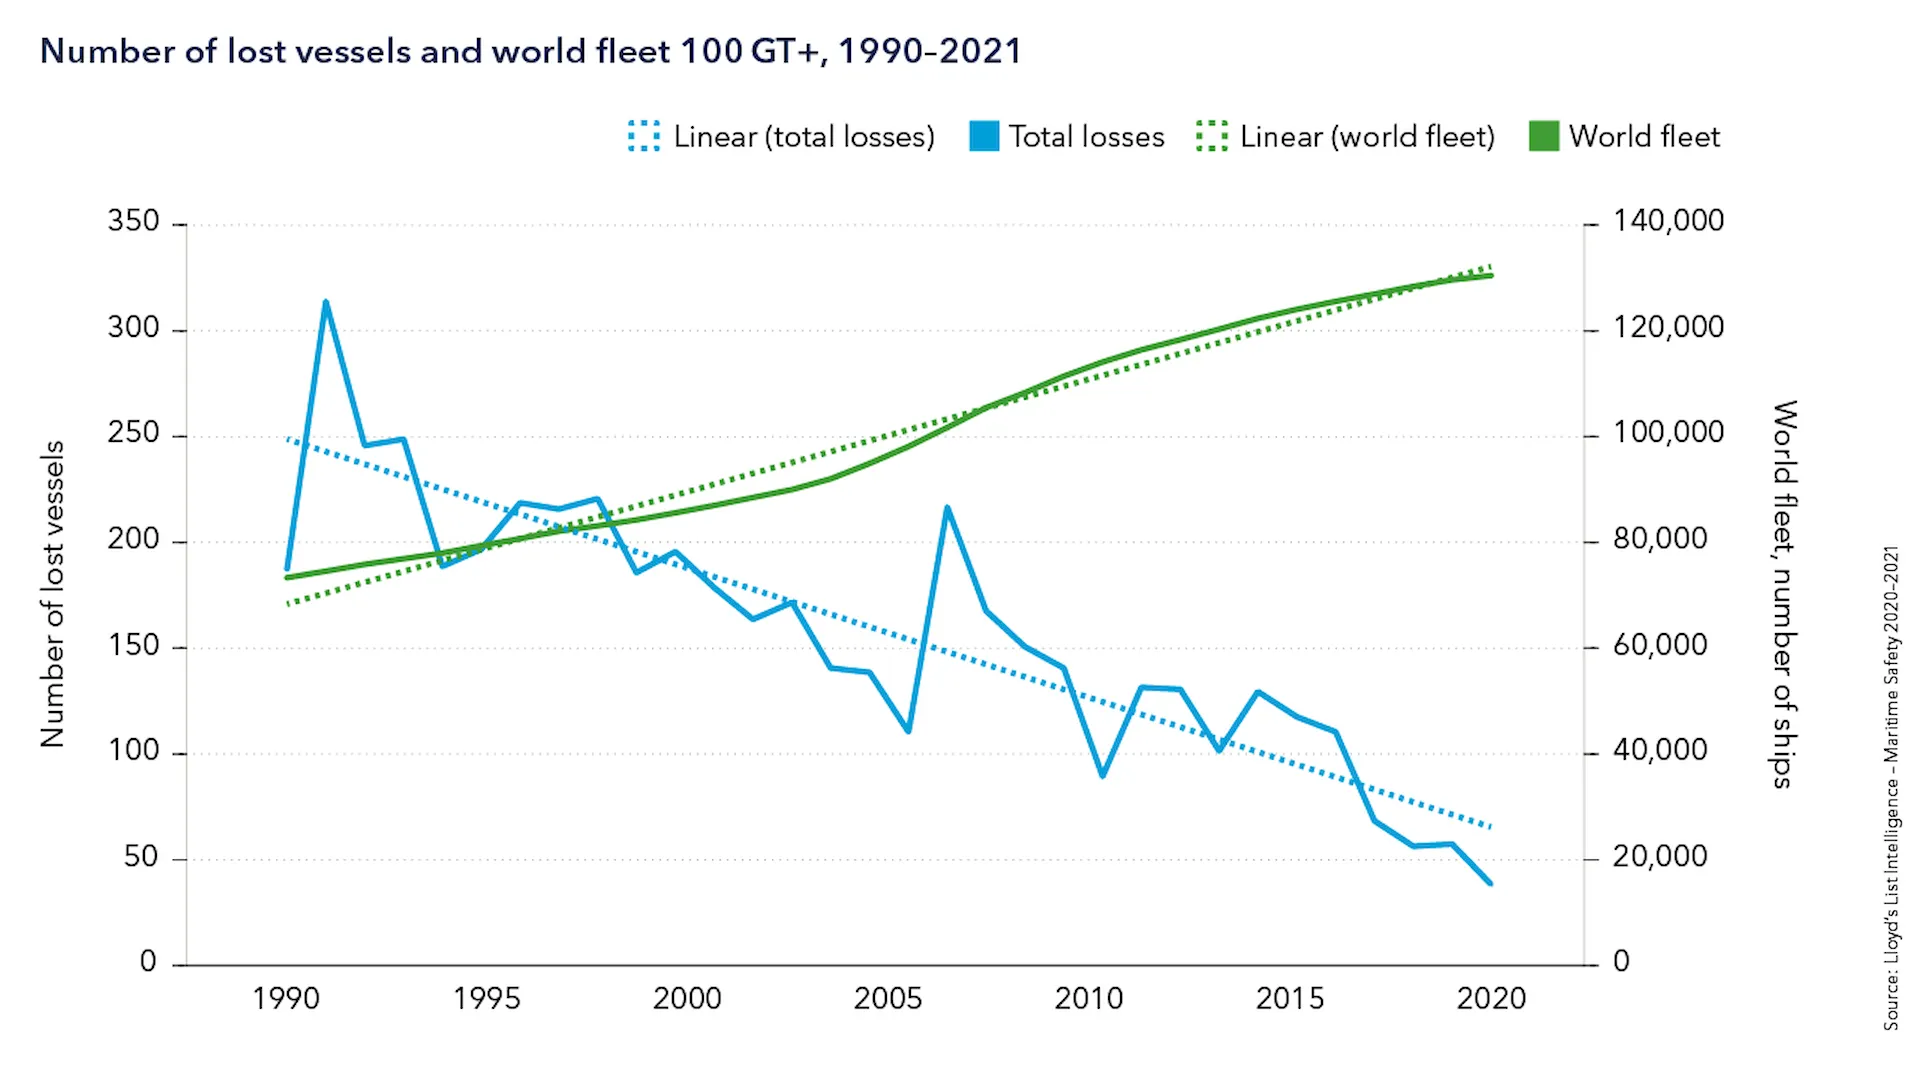
\includegraphics[width=0.65\linewidth]{images/number_of_lost_vessels.jpg.jpg}
    \caption{Grafik angka kecelakaan kapal dari tahun 1990 hingga 2020}
    \label{fig:pengurangan-kecelakaan-kapal}
\end{figure}


Apakah dengan kapal tersebut memiliki perangkat komputer terkoneksi dengan internet serta merta kapal tersebut terdigitalisasi atau kemudian risiko keselamatannya berkurang?. tentu saja tidak semudah itu, kembali ke analogi toko tadi maka tidak akan ada perubahan jika toko tersebut mempunyai perangkat komputer tapi tidak ada orang yang mengoperasikannya. Begitupun juga jika sudah ada manusia dan komputer namun tidak ada aturan main dan sistem yang mengatur apa yang harus dilakukan manusia di perangkat tersebut. Berdasarkan analogi sederhana tersebut dapat kita bayangkan elemen-elemen digitalisasi sebagai berikut:
\begin{itemize}
    \item Manusia: tanpa adanya yang mengoperasikan, perangkat komputer tidak terlalu berbeda dengan besi tua
    \item Perangkat Digital: ponsel, komputer, tablet dan sebagainya
    \item Sistem Digital: hal ini yang akan menyatukan dunia nyata dengan dunia digital dan mengatur bagaimana interaksi dua unsur yang lain.
\end{itemize}  



